\section{Research Description}
\label{sec:research}

\subsection{CPS Research Focus}

\FIXME{Here, we must ``identify and describe the specific core CPS research
areas being addressed in which novel and foundational research contributions
are being made."}

\subsection{Background and Related Work}
\label{sec:background}

\FIXME{This text is from 2018 proposal and needs to be updated.}

This research proposal builds on ideas, models, and techniques pioneered in two 
previous projects.
The first project, titled \emph{AMP}, created a prototype to redirect
daylight deeper into specific locations with a lightwell.
The building in which the prototype was installed is an 8~story factory
building built in 1895, in which a 5~story light well was cut out of
the floors. A skylight was located above the lightwell and provided the
daylight source.  The primary goal of the project was to develop and use
computational techniques to be able to reflect the rays of light into
the darker recesses of the lightwell. 
Figure~\ref{fig:raytracing} shows an example output from the resulting software
system (analyzing a hypothetical location).
A secondary goal of that work was to develop
a catoptric surface that connected to existing columns and beams, which was
divided into 300 reflective sub-surfaces to achieve the goal.
The project verified that the 300 custom geometrical sub-surfaces
could be designed and fabricated (see Figure~\ref{fig:amp}).
Though successful in its aims, an important limitation of the project
was that each reflective sub-surface had a fixed geometry.

\begin{figure}[ht]
\centering
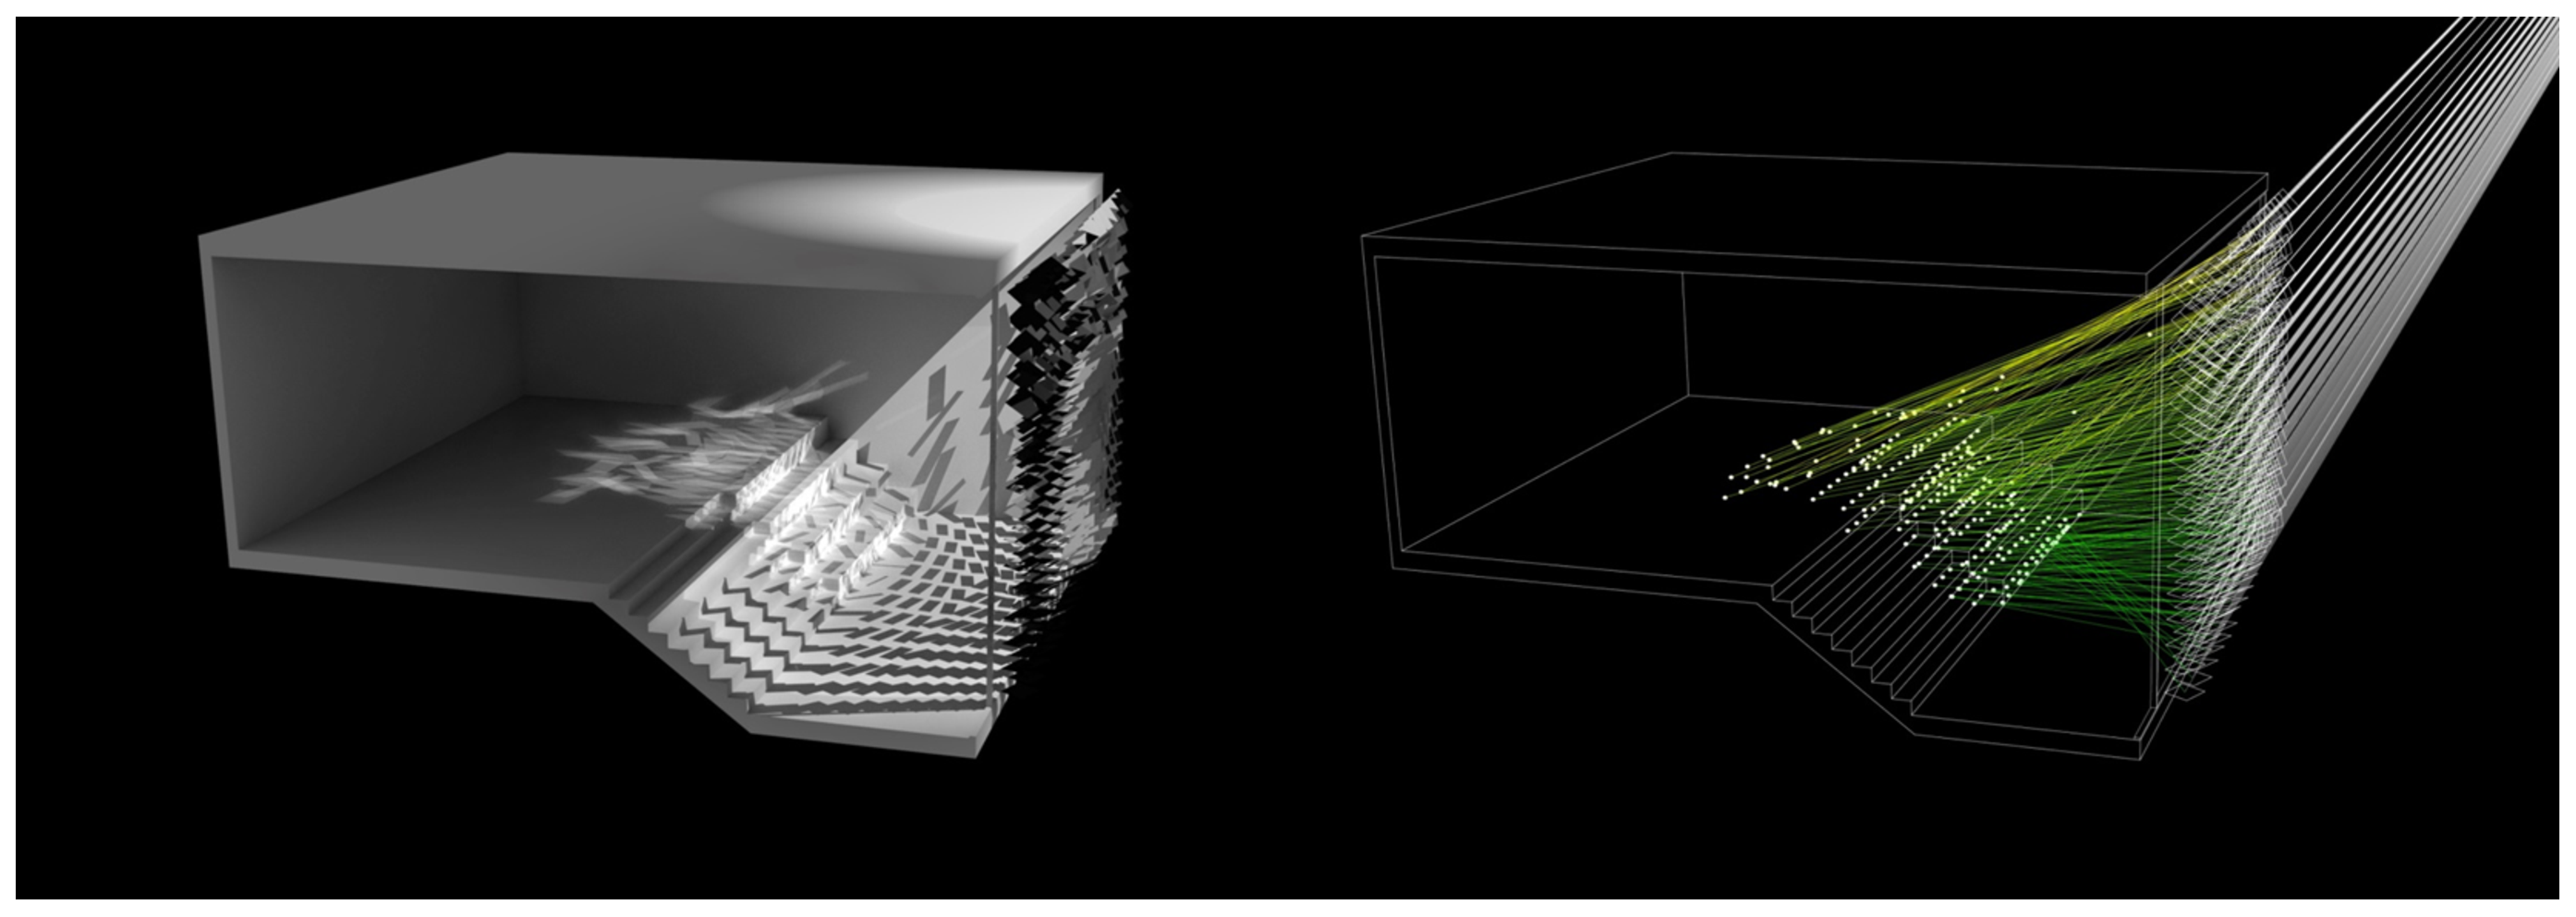
\includegraphics[width=0.95\linewidth]{figures/raytracing}
\caption{Ray tracing analysis of daylighting design.}
\label{fig:raytracing}
\end{figure}

The second project, titled \emph{Catoptric Surface: Steinberg prototype},
addressed that limitation of fixed geometry in AMP. The goal of this second
prototype was to create a series of mirrors that were independently
adjustable according to both the sun's position throughout the day and the desired
location within the building towards which to reflect the light. The ability to
vary the intensity of reflected daylight within the interior of a
building provides the occupants control of the light level for varying tasks
such as a lower light level required to read from a screen versus higher
light level for reading physical paper. This increased level of control
was enabled via the development of units providing 2 axes of rotation of each mirror
independently under software control. This second prototype provides a proof
of concept that individually controlled mirrors can effectively direct
daylight in a very controlled geometry. 
Figure~\ref{fig:steinberg2} shows a CAD illustration of the prototype,
and Figure~\ref{fig:steinberg} shows a photograph of a small number of
the installed mirrors.

\begin{figure}[ht]
\centering
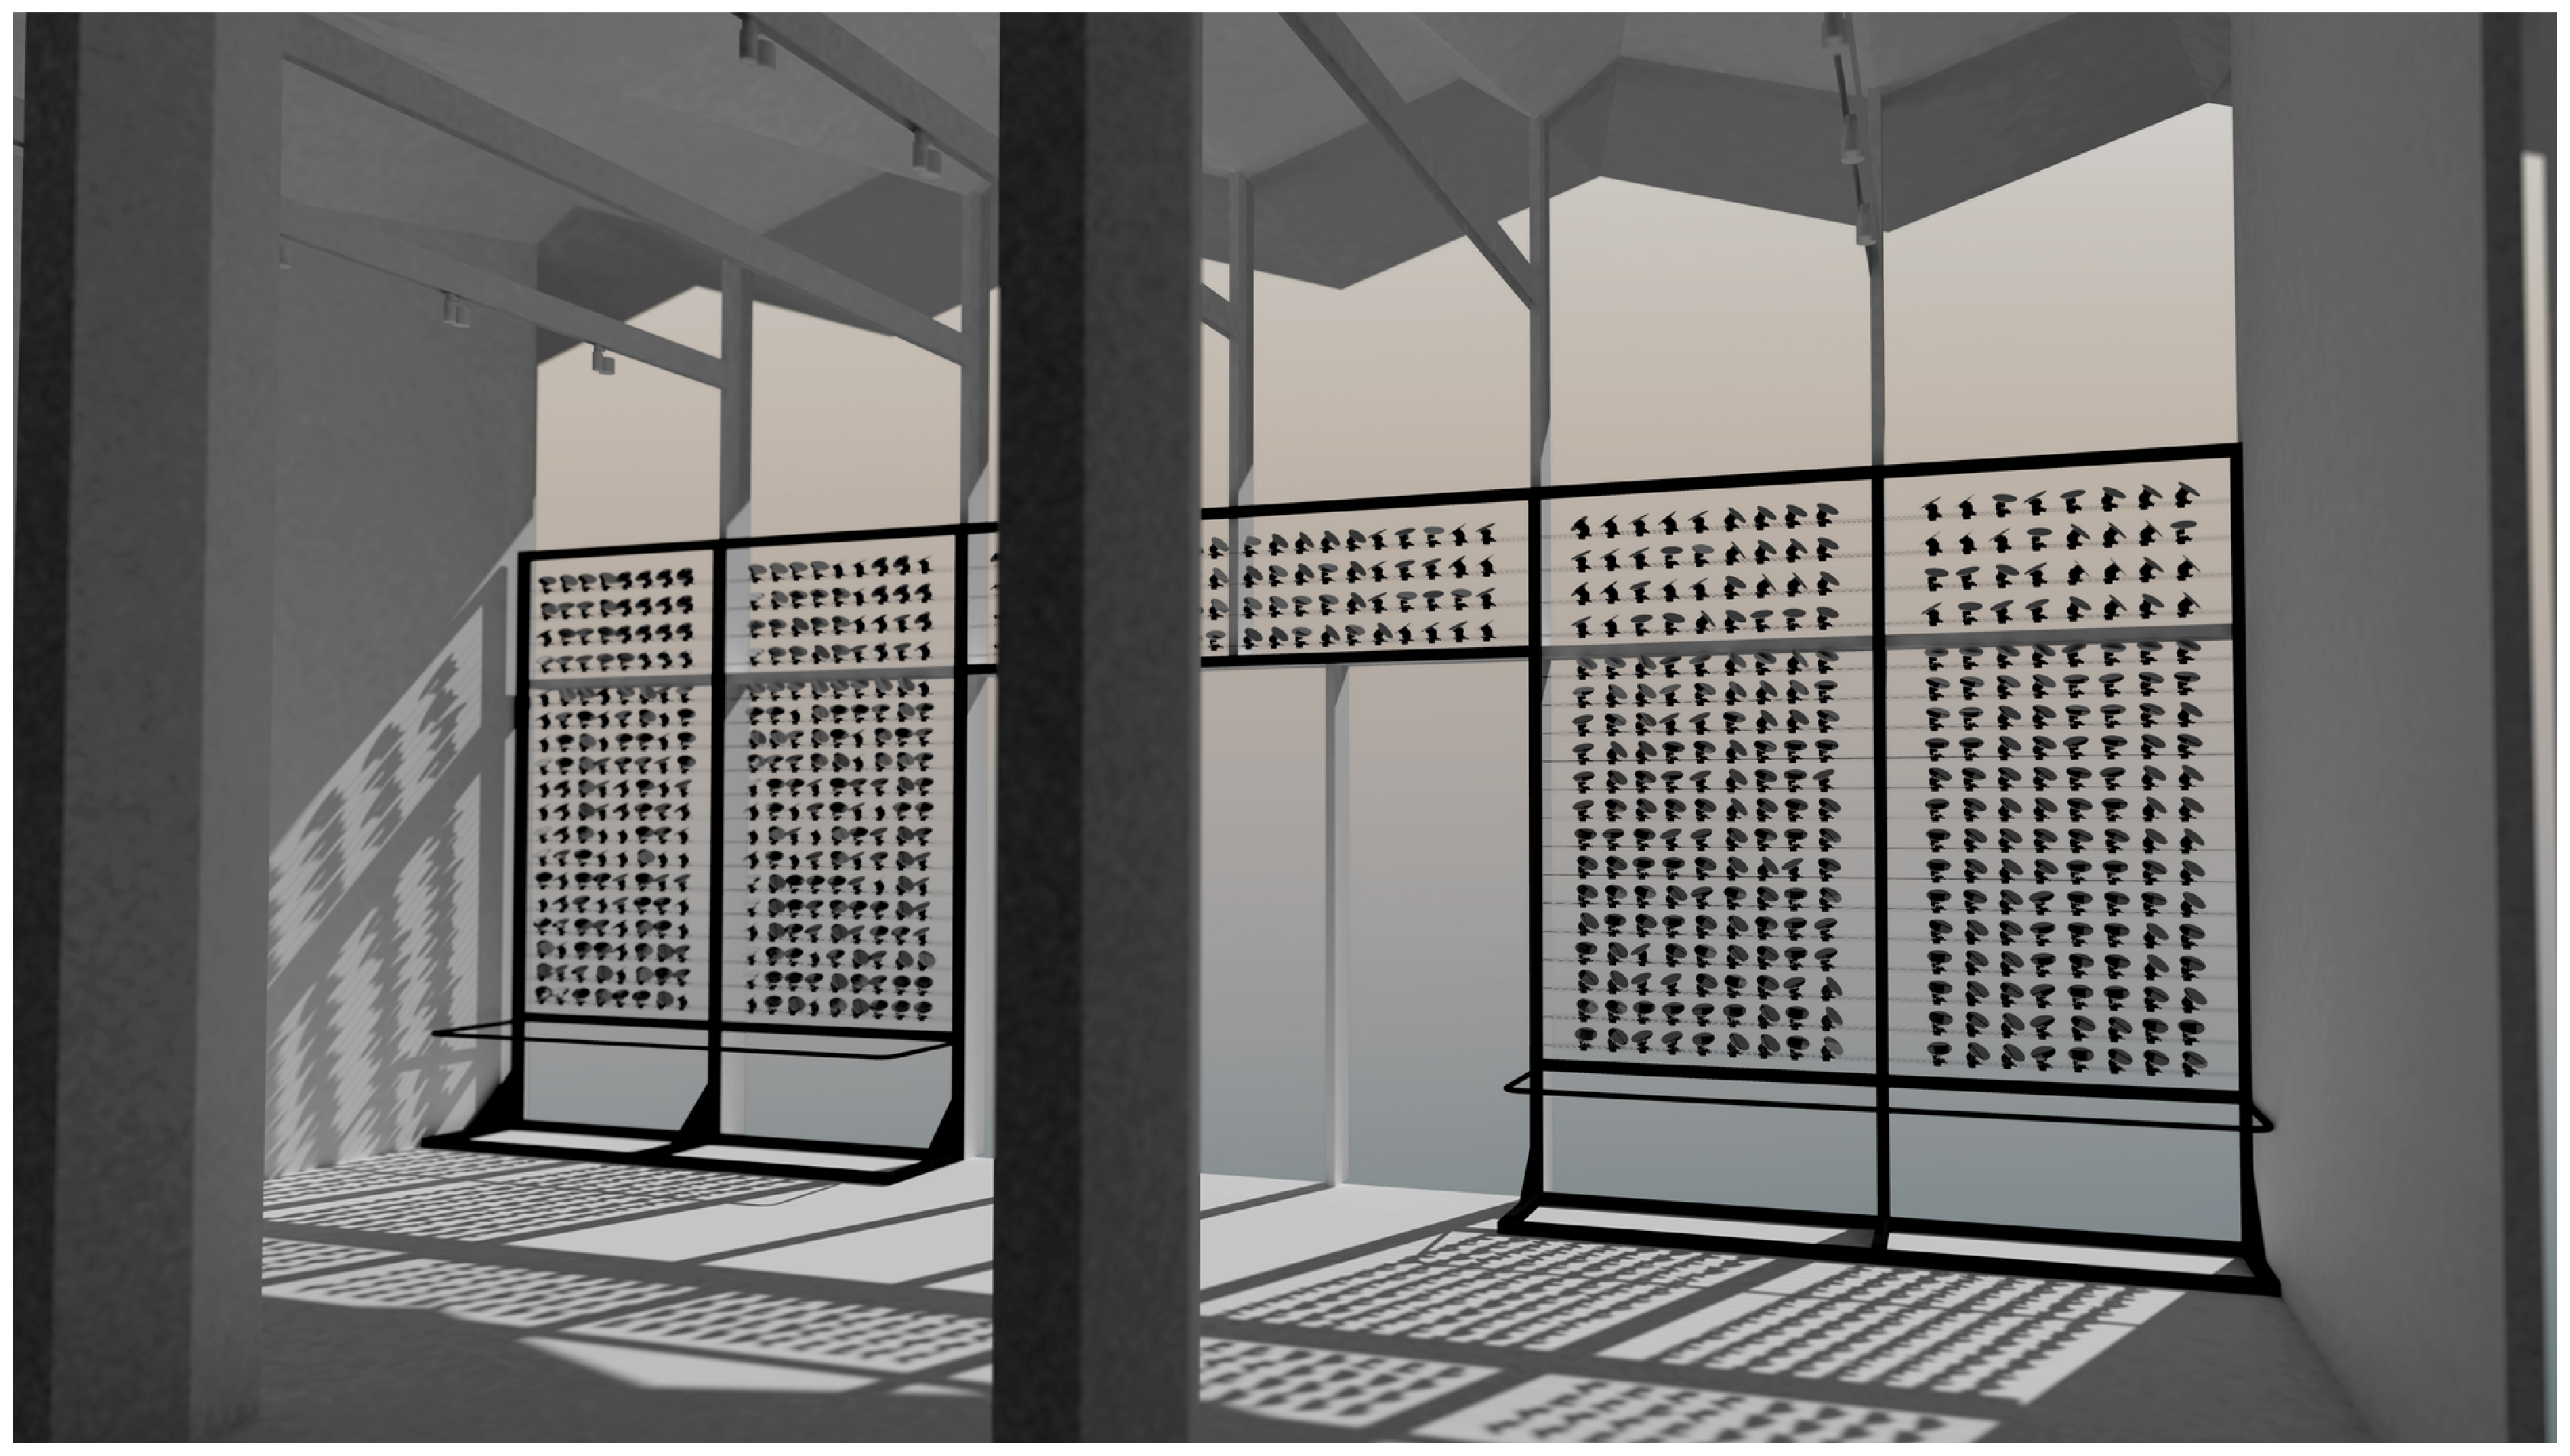
\includegraphics[width=0.9\linewidth]{figures/steinberg2}
\caption{CAD drawing of the Steinberg Hall prototype catoptric surface.}
\label{fig:steinberg2}
\end{figure}

Leslie~\cite{Leslie03} and Alrubaih et al.~\cite{azaise13} provide
a pair of review articles that effectively summarize current
approaches to daylighting in modern building design.
For the most part, these are passive systems, or might include
active control of shades~\cite{kt16}, with a strong emphasis on
achieving uniform, homogeneous illumination~\cite{bwkk15,gb16}.
Our emphasis is on dynamic control of the light position, with the explicit
intent to support inhomogeneous as well as homogeneous illumination patterns.

There have been a number of efforts to quantitatively model, and
empirically measure, prototype daylighting
systems~\cite{bwkk15,fsdm14,ls06,vm16,vgf+13}. A pair of studies, first by
Lee and Selkowitz~\cite{ls06} and followed by Fernandes et al.~\cite{fsdm14},
initially evaluated the potential for energy savings in the New York Times
Headquarters building and then measured the actual realized savings.

In this work, we will exploit Markov Decision Process (MDP)
theory~\cite{puterman} as a formal approach to optimize
catoptric surface control. MDPs represent a general approach
to modeling optimization problems and have been applied in a diverse set of
application areas~\cite{White93}: examples include robotics~\cite{ab10}, 
economics~\cite{bs98}, experiment design~\cite{kb85},
medical decisions~\cite{ahsr10}, manufacturing~\cite{yyl04},
agriculture~\cite{Kristensen03},
and our own group's use in real-time scheduling~\cite{gtsg08,tggs10}
and wireless spectrum management~\cite{mgc16}.

Our prior research has used Markov decision process
models~\cite{gtsg08} to generate resource management policies
off-line~\cite{gtgs09} for non-preemptive sharing of a resource
among multiple purposes at once on-line.  For example, a meter-tall robot's
camera (oriented by a pan-tilt unit similar to the ones we propose to
use in our multi-mirror catoptric installations) may be directed
downward to identify wire-frame chairs and other obstacles to
navigation that other sensors on the robot may have difficulty
detecting, or it may be directed upward to identify faces of people at
a social event whose images it can then capture. Given distributions of
the durations of intervals during which the camera would need to
remain pointed in a given direction to complete an individual task,
standard policy iteration techniques then can be used to generate
run-time policies that in expectation maximize an objective such as
adherence to a strictly proportional allocation of the resource over
time~\cite{gtsg08}, or even a more general definition of the utility 
of completing the different tasks at particular times~\cite{tggs10}.
We also showed that when different distributions of task completion
intervals can occur in different modes (e.g., when a robot moves
from room to room), it is possible to learn on-line what mode
the system is in, or if the mode is known what the distributions are,
but not both~\cite{gtgsuai10}.

However, policy iteration is exponentially expensive in its computational
requirements, and even the memory requirements to store complete policies 
for on-line use may be prohibitive in resource-limited systems.  We 
therefore focused next on the policies that were being generated from 
the models, and discovered consistent structure in those policies that 
allowed a reasonable heuristic approximation.  For simple proportional 
sharing, a single geometric partition of a simplex could be calibrated 
to encode the appropriate policy accurately~\cite{gtspmgs10}.
For utility-based resource sharing multiple disjoint heuristics were needed but
the most effective one to use was clearly defined by problem parameters~\cite{tblwgs11}.

As a further illustration both of the applicability of MDP-based
policy iteration to generate effective resource management policies,
we applied similar techniques to manage another dissimilar resource: 
the transmission spectrum in wireless networks~\cite{mskgct13}.  
Although the semantics of that resource differed radically from the pan-tilt camera, 
the MDP models were reasonably similar.  We extended the basic model to
include modulation as well as admission decisions, discovered and characterized
common structure among the policies that were generated, and again obtained
efficient and effective heuristic policies for on-line use~\cite{mgc16}.

In this proposal we adopt the definition used in our prior work~\cite{gtsg08}
of a (discrete-time) Markov decision process as a 5-tuple
$(\mathcal{X}, \mathcal{A}, T, R, \gamma)$, with \emph{states} designated
as $\chi \in \mathcal{X}$, \emph{actions} designated as $a \in \mathcal{A}$,
and a transition system, $T$, which gives the probability
$P_T (\chi' \mid \chi, a)$ of transitioning from state $\chi$ to
state $\chi'$ on action $a$.
The reward function $R(\chi, a, \chi') \in \mathbb R_{\ge 0}$ describes the
reward that accrues when transitioning from state $\chi$ to
state $\chi'$ via action $a$, under a discount factor, $\gamma$,
to ensure convergence of the long term reward.
In what follows, we will explain how we plan to exploit the formal theory of 
MDPs as an approach to optimization of the configuration of catoptric surfaces.

\subsection{Research Questions}

\subsection{Intellectual Merit}

\FIXME{This section is strictly required. One option is to use it to summarize
the research directions. Another option is to merge it with the section
above, which articulates the research questions we want to address and how
we will go about tackling them. If we do the latter, we must maintain
\emph{this} section title.}
